\chapter{Measurements}\label{chap:measurements}

In order to test the detector and crystal response, multiple electronic setups were used to obtain spectra from calibrated sources along with other interesting measurements. This chapter summarizes the most important measurements achieved at the time of publication.

\section{Rohde\&Schwarz RTO6 oscilloscope}

The Rohde\&Schwarz RTO6 oscilloscope was the main troubleshooting tool used to test the detector as a whole and measure spectra in order to calibrate the crystal response while coupled with a SiPM. Figure \ref{fig:RS_spectra} shows the spectra obtained with the histogram functionality of the oscilloscope for each isotope used to calibrate the detector. 

\begin{figure}
    \begin{subfigure}[t]{0.48\textwidth}
      \centering
      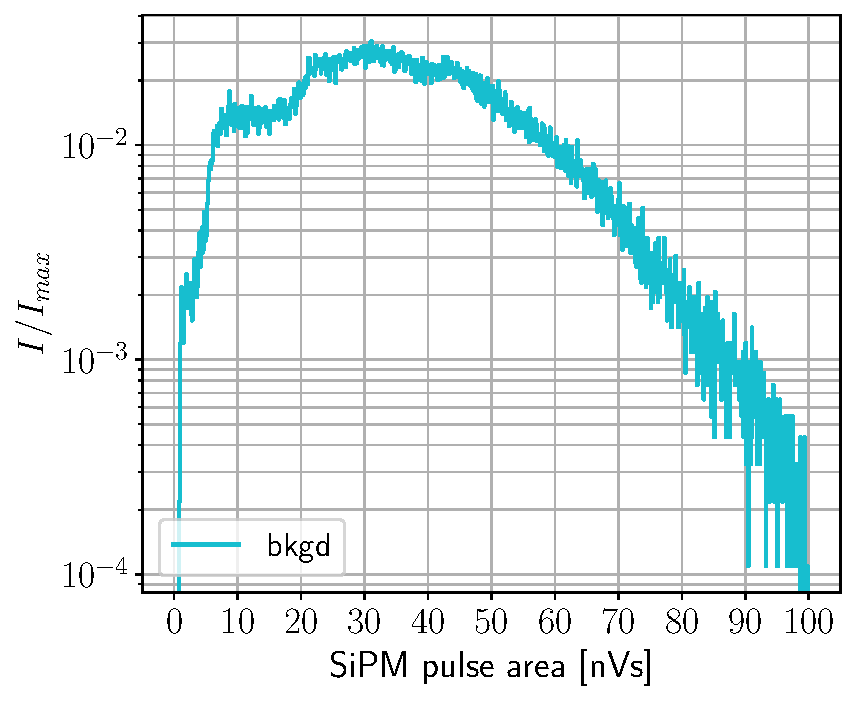
\includegraphics[width=\textwidth]{measurements/RS/teflon-bkgd.pdf}
      \caption{\label{sfig:RS_bkgd}LYSO background.}
    \end{subfigure}
    \hfill
    \begin{subfigure}[t]{0.48\textwidth}
      \centering
      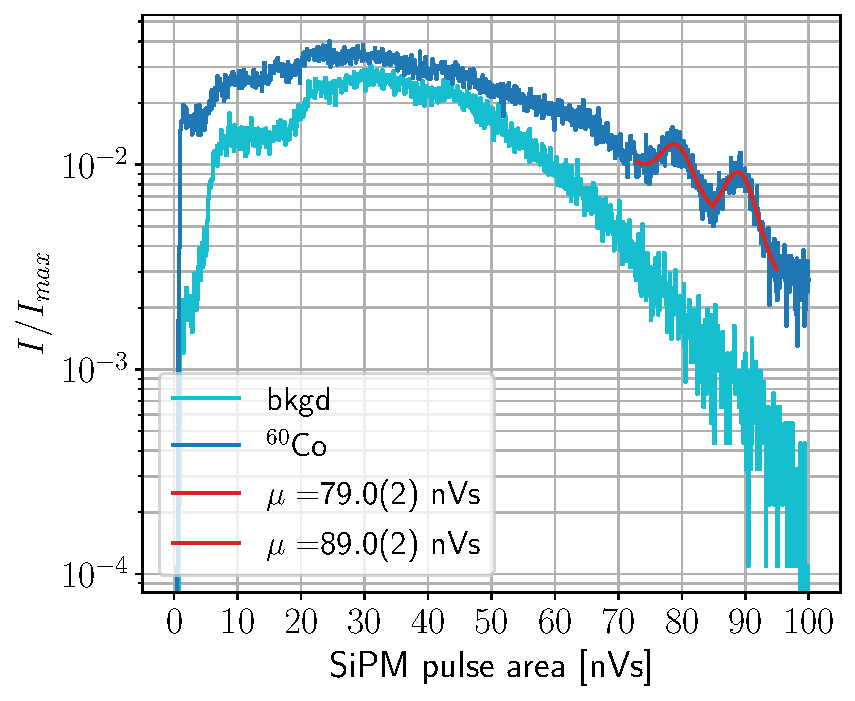
\includegraphics[width=\textwidth]{measurements/RS/teflon-side-Co60.pdf}
      \caption{\label{sfig:RS_60Co}$^{60}$Co.}
    \end{subfigure}
    \medskip
    \begin{subfigure}[t]{0.48\textwidth}
      \centering
      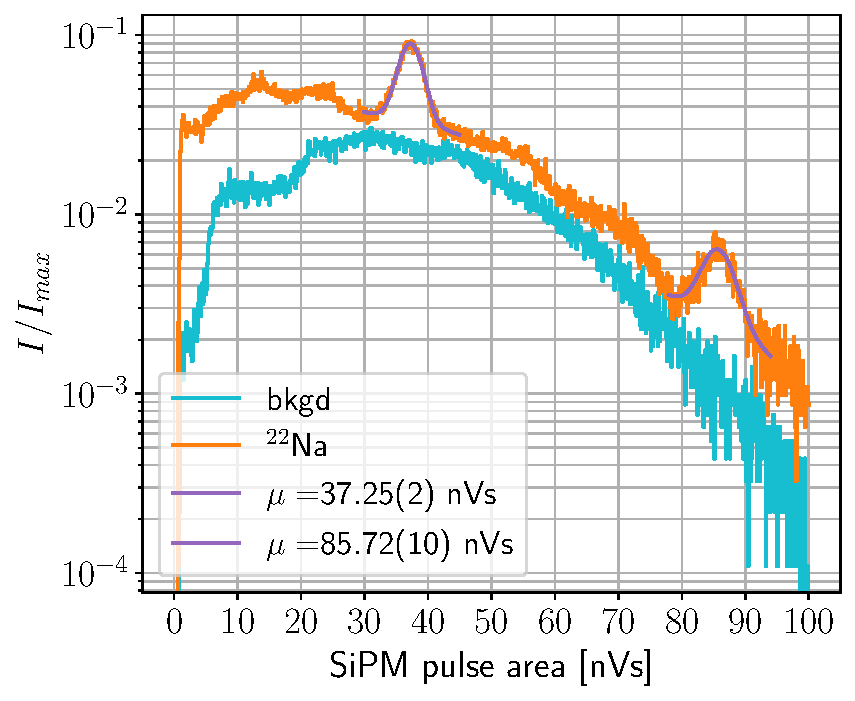
\includegraphics[width=\textwidth]{measurements/RS/teflon-side-Na22.pdf}
      \caption{\label{sfig:RS_22Na}$^{22}$Na.}
    \end{subfigure}
    \hfill
    \begin{subfigure}[t]{0.48\textwidth}
      \centering
      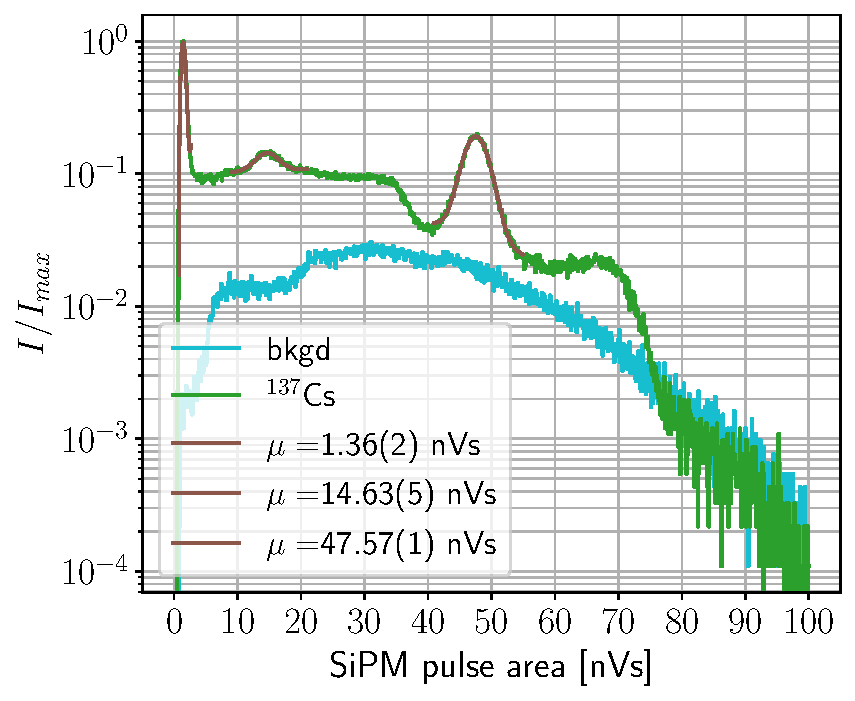
\includegraphics[width=\textwidth]{measurements/RS/teflon-side-Cs137.pdf}
      \caption{\label{sfig:RS_137Cs}$^{137}$Cs.}
    \end{subfigure}
    \caption{\label{fig:RS_spectra}Spectra measured with the histogram functionality of a Rohde\&Schwarz RTO6 oscilloscope. The $x$ axis measures SiPM pulse areas since the oscilloscope creates histograms based on the area under each pulse such as those shown in \ref{fig:signal_processing}. Each graph features the centroid of the Gaussian fitted to each peak.}
  \end{figure}

It is important to note here the shape of the background, remembering Figure \ref{fig:LYSO_background}, a sudden increase in intensity should occur at around 290 and 597 \unit{\kilo\eV}, therefore the 511 \unit{\kilo\eV} peak of $^{22}$Na should lie in between these values, while 662 \unit{\kilo\eV} from $^{137}$Cs would lie above the second increase in background counts. These approximations can help us get a notion of what we are seeing in the various spectra illustrated in Fig. \ref{fig:RS_spectra}.

The highest peak in $^{137}$Cs is presumed to be caused by x-ray emissions from lower shell electrons filling the space left by internal conversion electrons, this peak is also featured in Figure \ref{fig:Cs137_description}. One important feature in the cesium spectrum is the relatively high intensities passed the photoelectric peak (at 47.57(1) nVs according to the gaussian fit), this is not due to LYSO background however since these counts greatly exceed the expected background.

Fitting gaussian functions to the main peaks one can get the relation between energy and pulse area (Fig. \ref{sfig:RS_LYSO_calibration_low_peaks}) based on the decay schemes shown in Figure \ref{fig:decay_schemes}. Considering the x-ray and backscattering peaks of $^{137}$Cs, however, seems to cause an overestimation of the energies, as can be seen in Figure \ref{sfig:RS_LYSO_calibrated_spectrum_low_peaks}, where the pair-production peak of sodium, for example, lies at 535.95 keV instead of 511 keV. The calibration shown in Figure \subref{sfig:RS_LYSO_calibration} does not take into account the troublesome peaks of cesium, better estimating high energy peaks, this however results in negative-energy predictions at the lower energy range in the spectrum.

\begin{figure}[H]
  \begin{subfigure}[t]{\textwidth}
    \centering
    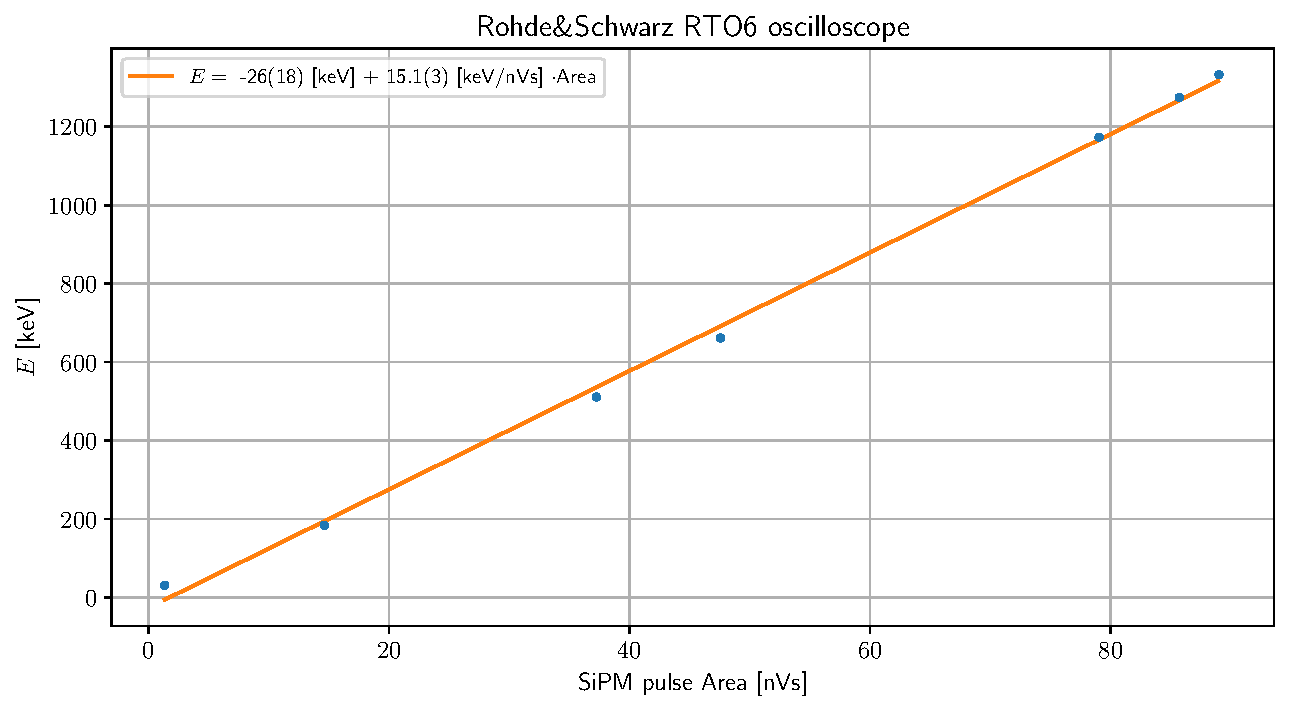
\includegraphics[width=.98\textwidth]{measurements/RS/LYSO_calibration_low_peaks.pdf}
    \caption{\label{sfig:RS_LYSO_calibration_low_peaks}LYSO calibration from Rohde\&Schwarz oscilloscope. Obtained by fitting gaussian functions to the main peaks shown in Fig \ref{sfig:RS_60Co}, \subref{sfig:RS_22Na}, and \subref{sfig:RS_137Cs}.}
  \end{subfigure}
  \medskip
  \begin{subfigure}[t]{\textwidth}
    \centering
    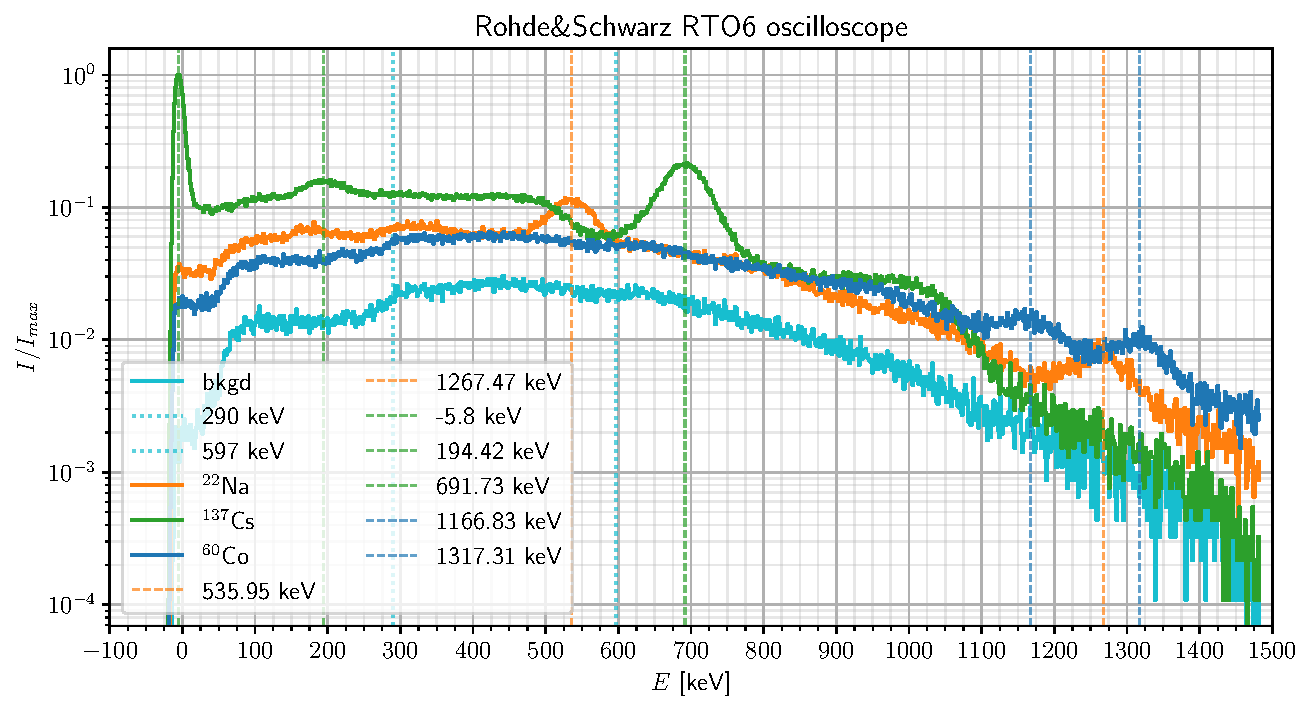
\includegraphics[width=.98\textwidth]{measurements/RS/Calibrated_spectrum_low_peaks.pdf}
    \caption{\label{sfig:RS_LYSO_calibrated_spectrum_low_peaks}Calibrated spectrum obtained from the channel-energy conversion shown in \subref{sfig:RS_LYSO_calibration_low_peaks}.}
  \end{subfigure}
  \caption{\label{fig:RS_low_peaks_calibration}Calibrated spectrum taking into account the x-ray and backscattering peaks of $^{137}$Cs.}
\end{figure}

\begin{figure}[H]
  \begin{subfigure}[t]{\textwidth}
    \centering
    \includegraphics[width=.98\textwidth]{measurements/RS/LYSO_calibration.pdf}
    \caption{\label{sfig:RS_LYSO_calibration}LYSO calibration from Rohde\&Schwarz oscilloscope. Excluding x-ray and backscattering peaks from \subref{sfig:RS_137Cs}.}
  \end{subfigure}
  \medskip
  \begin{subfigure}[t]{\textwidth}
    \centering
    \includegraphics[width=.98\textwidth]{measurements/RS/Calibrated_spectrum.pdf}
    \caption{\label{sfig:RS_LYSO_calibrated_spectrum}Calibrated spectrum obtained from the channel-energy conversion shown in \subref{sfig:RS_LYSO_calibration}.}
  \end{subfigure}
  \caption{\label{fig:RS_calibration}Calibrated spectrum, ignoring the x-ray and backscattering peaks of $^{137}$Cs.}
\end{figure}


\section{CosmicWatch electronics}

\section{NIM modules}

In the same way the CosmicWatch was studied with the Rohde\&Schwarz oscilloscope, NIM modules were used to get a LYSO calibration when coupled with the SiPM, this section shows some of the results obtained.

It is important to note some of the odd features in these spectra. $^{54}$Mn, like $^{137}$Cs, is a monoenergetic source, meaning that it mostly produces only one gamma ray, in this case at 834.848 \unit{\kilo\eV}, which lies slightly above 662 \unit{\kilo\eV} ($^{137}$Cs), therefore, the peak in channel 259 should correspond to the gamma emission from Manganese. However, there is again a very high number of events above this energy. Aside from this, it is also clear that the shape of this peak does not fully adjust to a gaussian distribution, showing that there is an underlying structure that has not been explained. These odd features can also be seen in $^{137}$Cs.

In principle, $^{68}$Ge should have a spectrum very similar to $^{22}$Na, since it also decays through $\beta^+$ to excited states of $^{68}$Ga, which emit high energy gammas. In this case, however, the decay chain most often ends in a stable state of $^{68}$Zn, this means that the only appreciable peak should lie at 511 \unit{\kilo\eV} due to positron annihilation, agreeing with Fig. \ref{sfig:NIM_68Ge}. Notably in Figure \ref{sfig:NIM_68Ge} there are very few counts at energies above 511 \unit{\kilo\eV}, but this must be due to the low activity of the source used. 

\begin{figure}
  \begin{subfigure}[t]{0.47\textwidth}
    \centering
    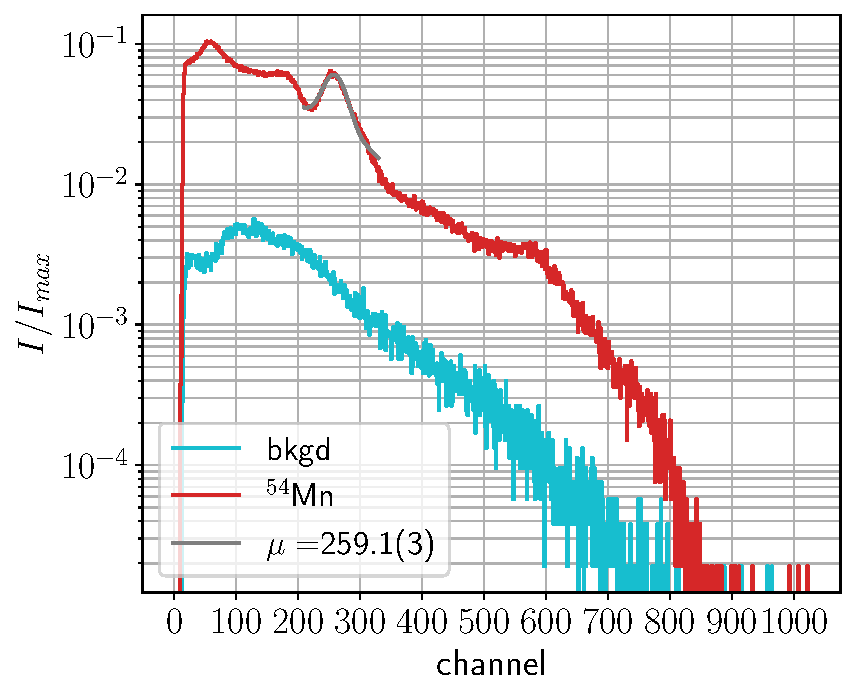
\includegraphics[width=\textwidth]{measurements/NIM/54Mn.pdf}
    \caption{\label{sfig:NIM_54Mn}$^{54}$Mn.}
  \end{subfigure}
  \hfill
  \begin{subfigure}[t]{0.47\textwidth}
    \centering
    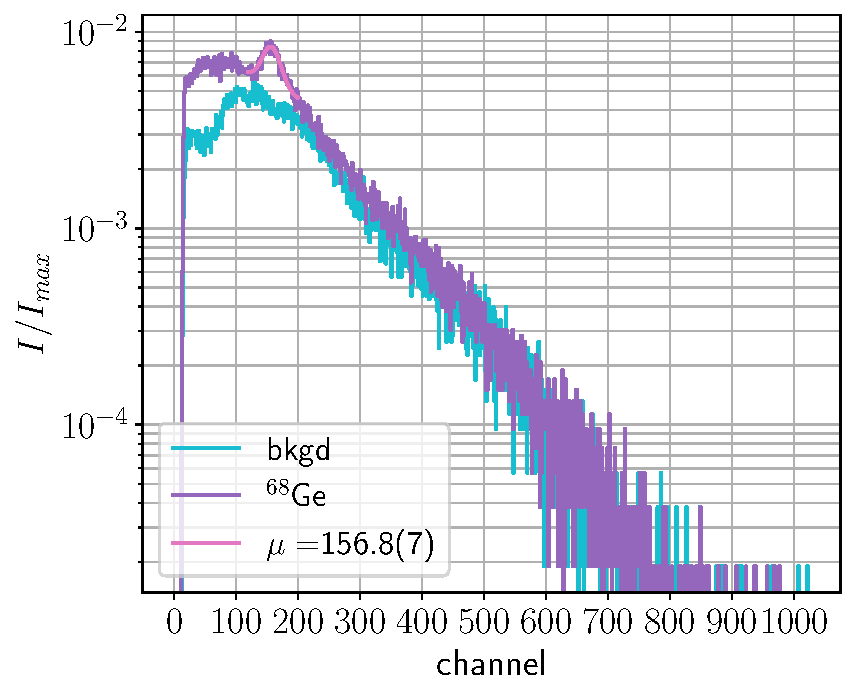
\includegraphics[width=\textwidth]{measurements/NIM/68Ge.pdf}
    \caption{\label{sfig:NIM_68Ge}$^{68}$Ge.}
  \end{subfigure}
  \medskip
  \begin{subfigure}[t]{0.47\textwidth}
    \centering
    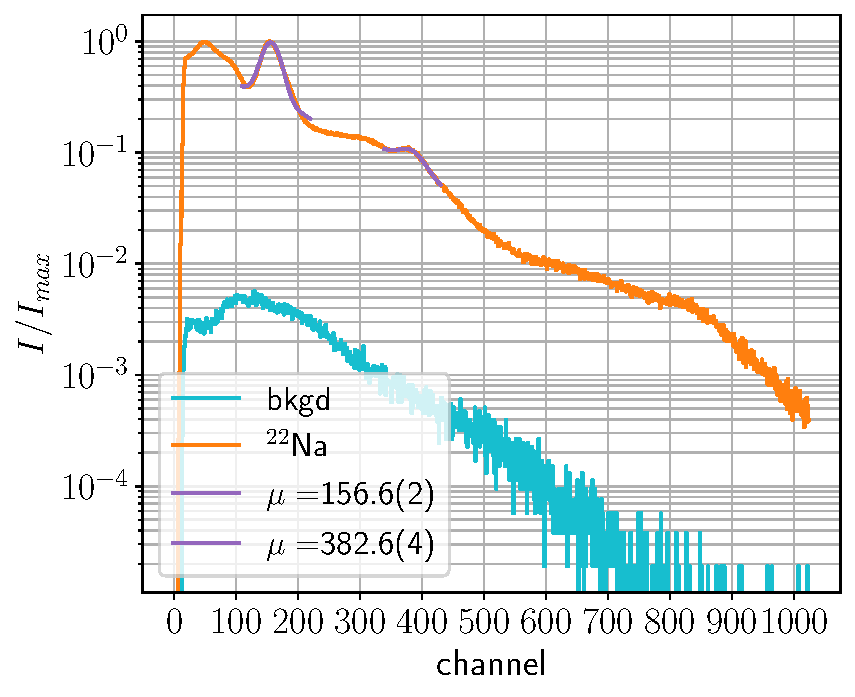
\includegraphics[width=\textwidth]{measurements/NIM/22Na.pdf}
    \caption{\label{sfig:NIM_22Na}$^{22}$Na.}
  \end{subfigure}
  \hfill
  \begin{subfigure}[t]{0.47\textwidth}
    \centering
    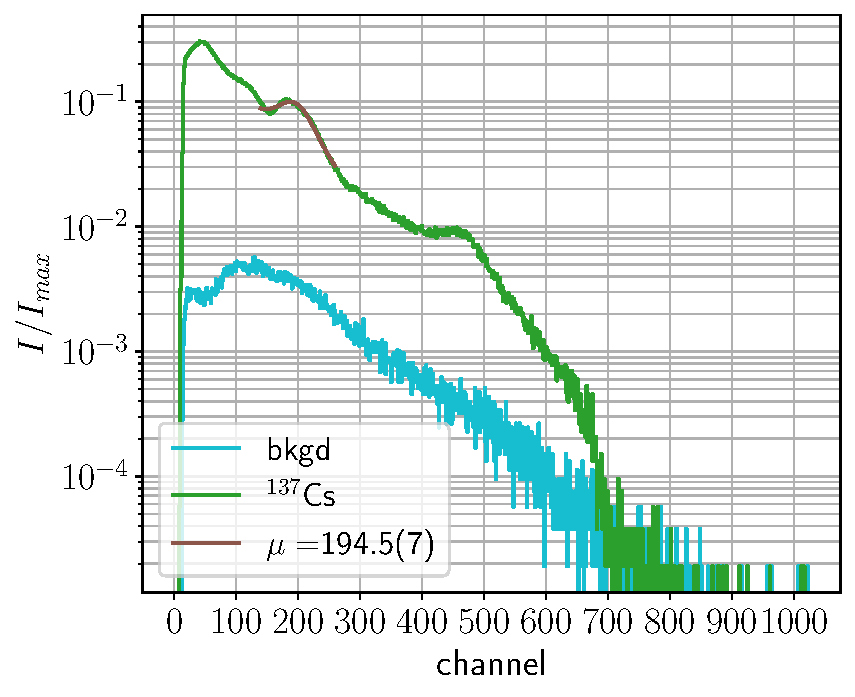
\includegraphics[width=\textwidth]{measurements/NIM/137Cs_HA.pdf}
    \caption{\label{sfig:NIM_137Cs}$^{137}$Cs.}
  \end{subfigure}
  \caption{\label{fig:NIM_spectra}Spectra measured with a Time Filter Amplifier and Analog to Digital Converter NIM modules. The $x$ axis measures channels since the ADC creates a histogram based on pulse area. Each graph features the centroid of the Gaussian fitted to each peak.}
\end{figure}

\begin{figure}[H]
  \begin{subfigure}[t]{\textwidth}
    \centering
    \includegraphics[width=.98\textwidth]{measurements/NIM/LYSO_calibration.pdf}
    \caption{\label{sfig:NIM_LYSO_calibration}LYSO calibration from NIM modules. Obtained by fitting gaussian functions to the main peaks shown in Fig \ref{sfig:NIM_54Mn} to \subref{sfig:NIM_137Cs}.}
  \end{subfigure}
  \medskip
  \begin{subfigure}[t]{\textwidth}
    \centering
    \includegraphics[width=.98\textwidth]{measurements/NIM/Calibrated_spectrum.pdf}
    \caption{\label{sfig:NIM_LYSO_calibrated_spectrum}Calibrated spectrum obtained from the channel-energy conversion shown in \subref{sfig:NIM_LYSO_calibration}.}
  \end{subfigure}
  \caption{\label{fig:NIM_calibration}Calibrated spectrum.}
\end{figure}

Notably, this new calibration does not result in the prediction of negative energies despite the various flaws in these spectra.

\section{Variable crystal size}\label{sec:LYSO_size}

\begin{figure}
  \begin{subfigure}[t]{0.49\textwidth}
    \centering
    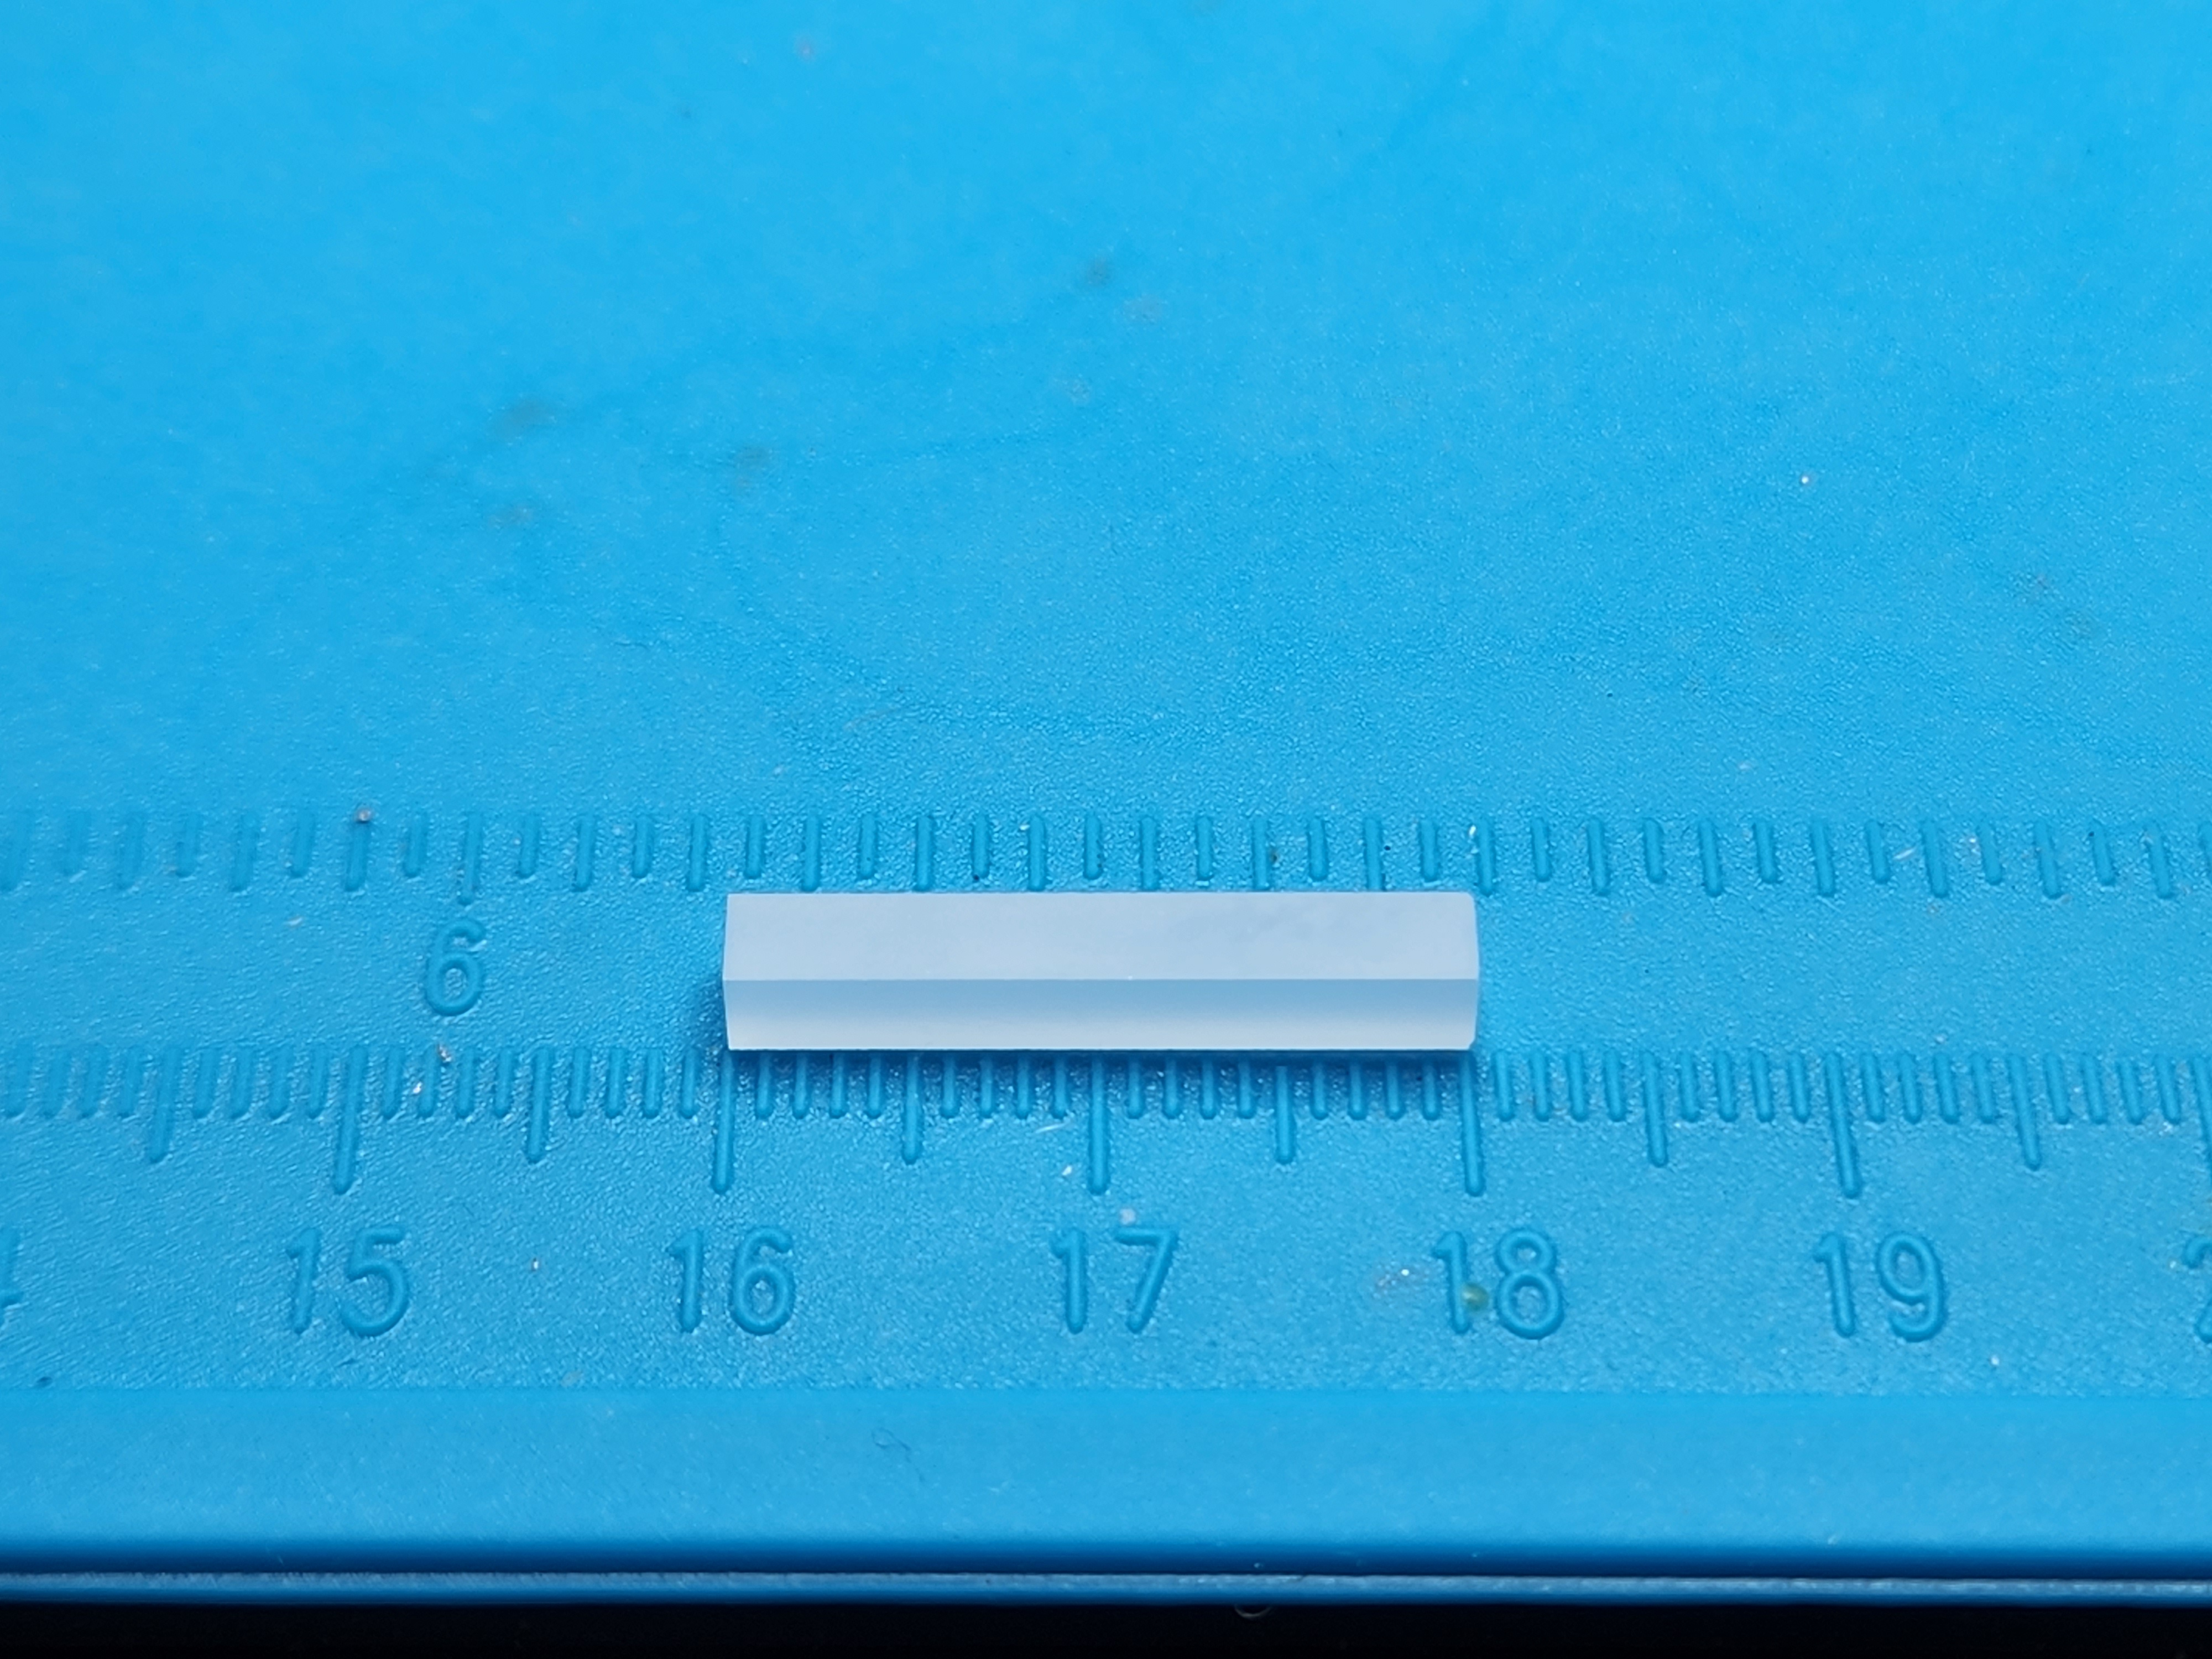
\includegraphics[width=\textwidth]{measurements/LYSO_crystals/LYSO_20_3_3.jpg}
  \end{subfigure}
  \begin{subfigure}[t]{0.49\textwidth}
    \centering
    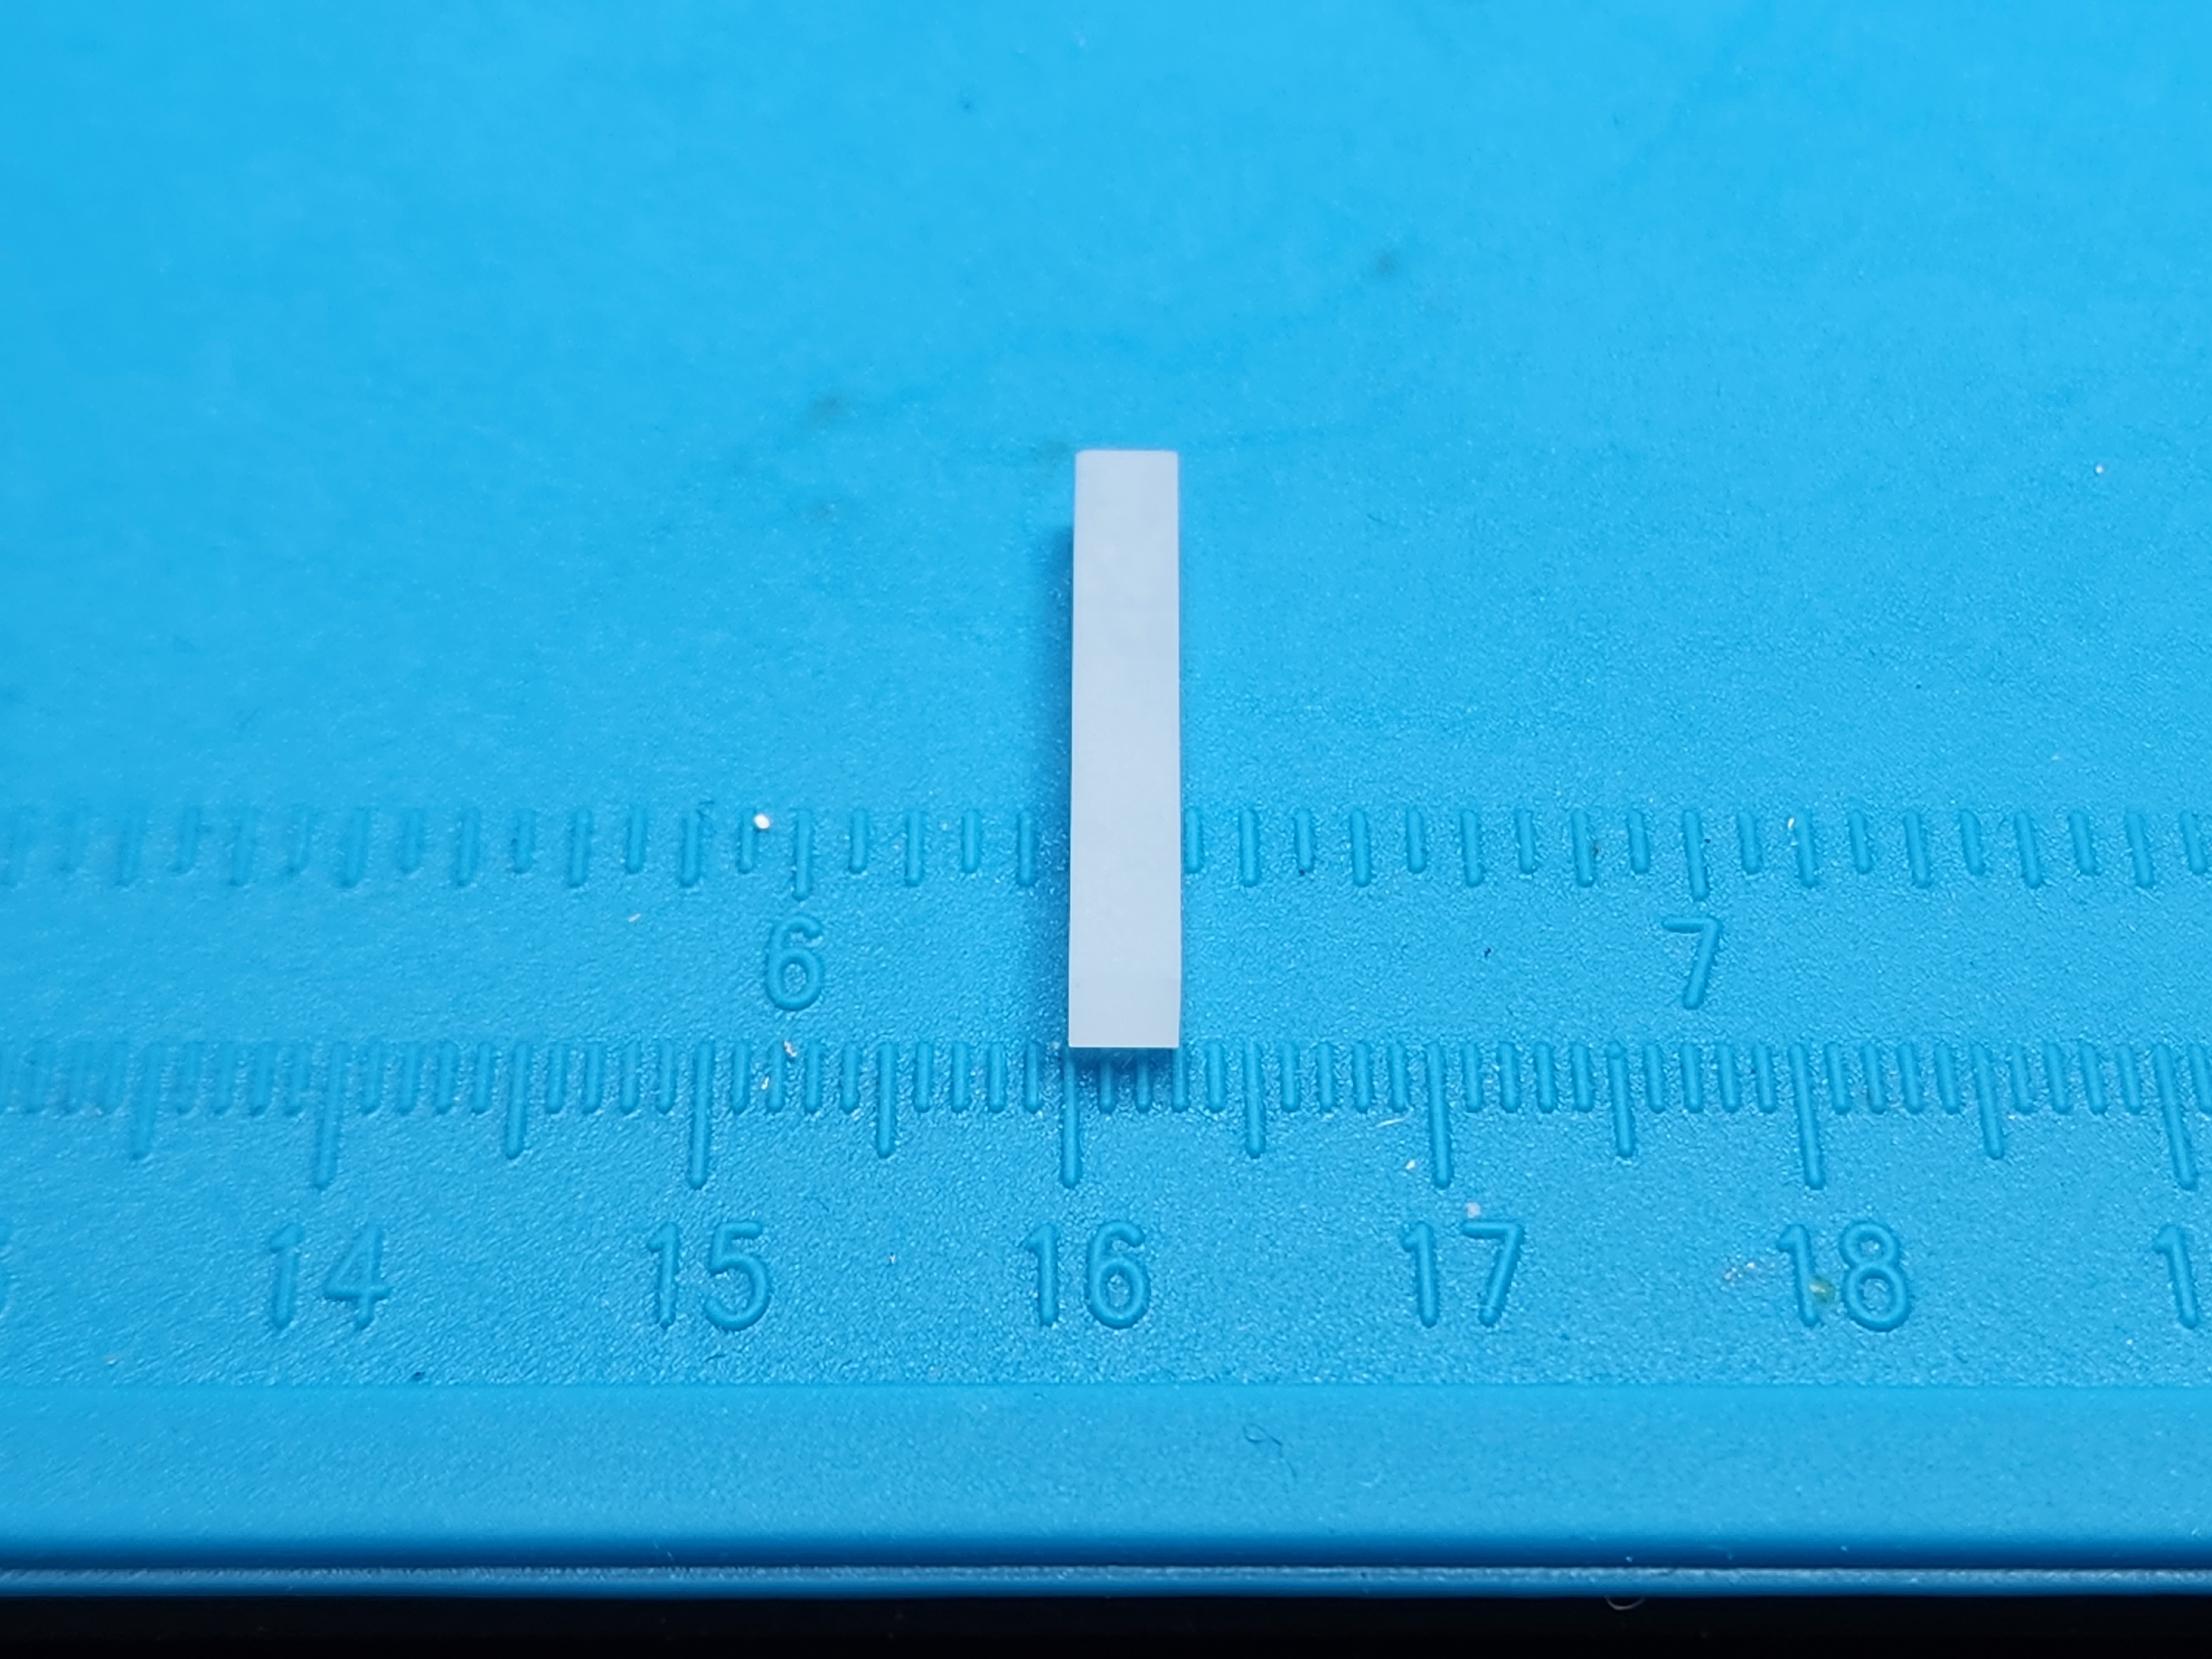
\includegraphics[width=\textwidth]{measurements/LYSO_crystals/LYSO_20_3_3_2.jpg}
  \end{subfigure}
  \medskip
  \begin{subfigure}[t]{0.49\textwidth}
    \centering
    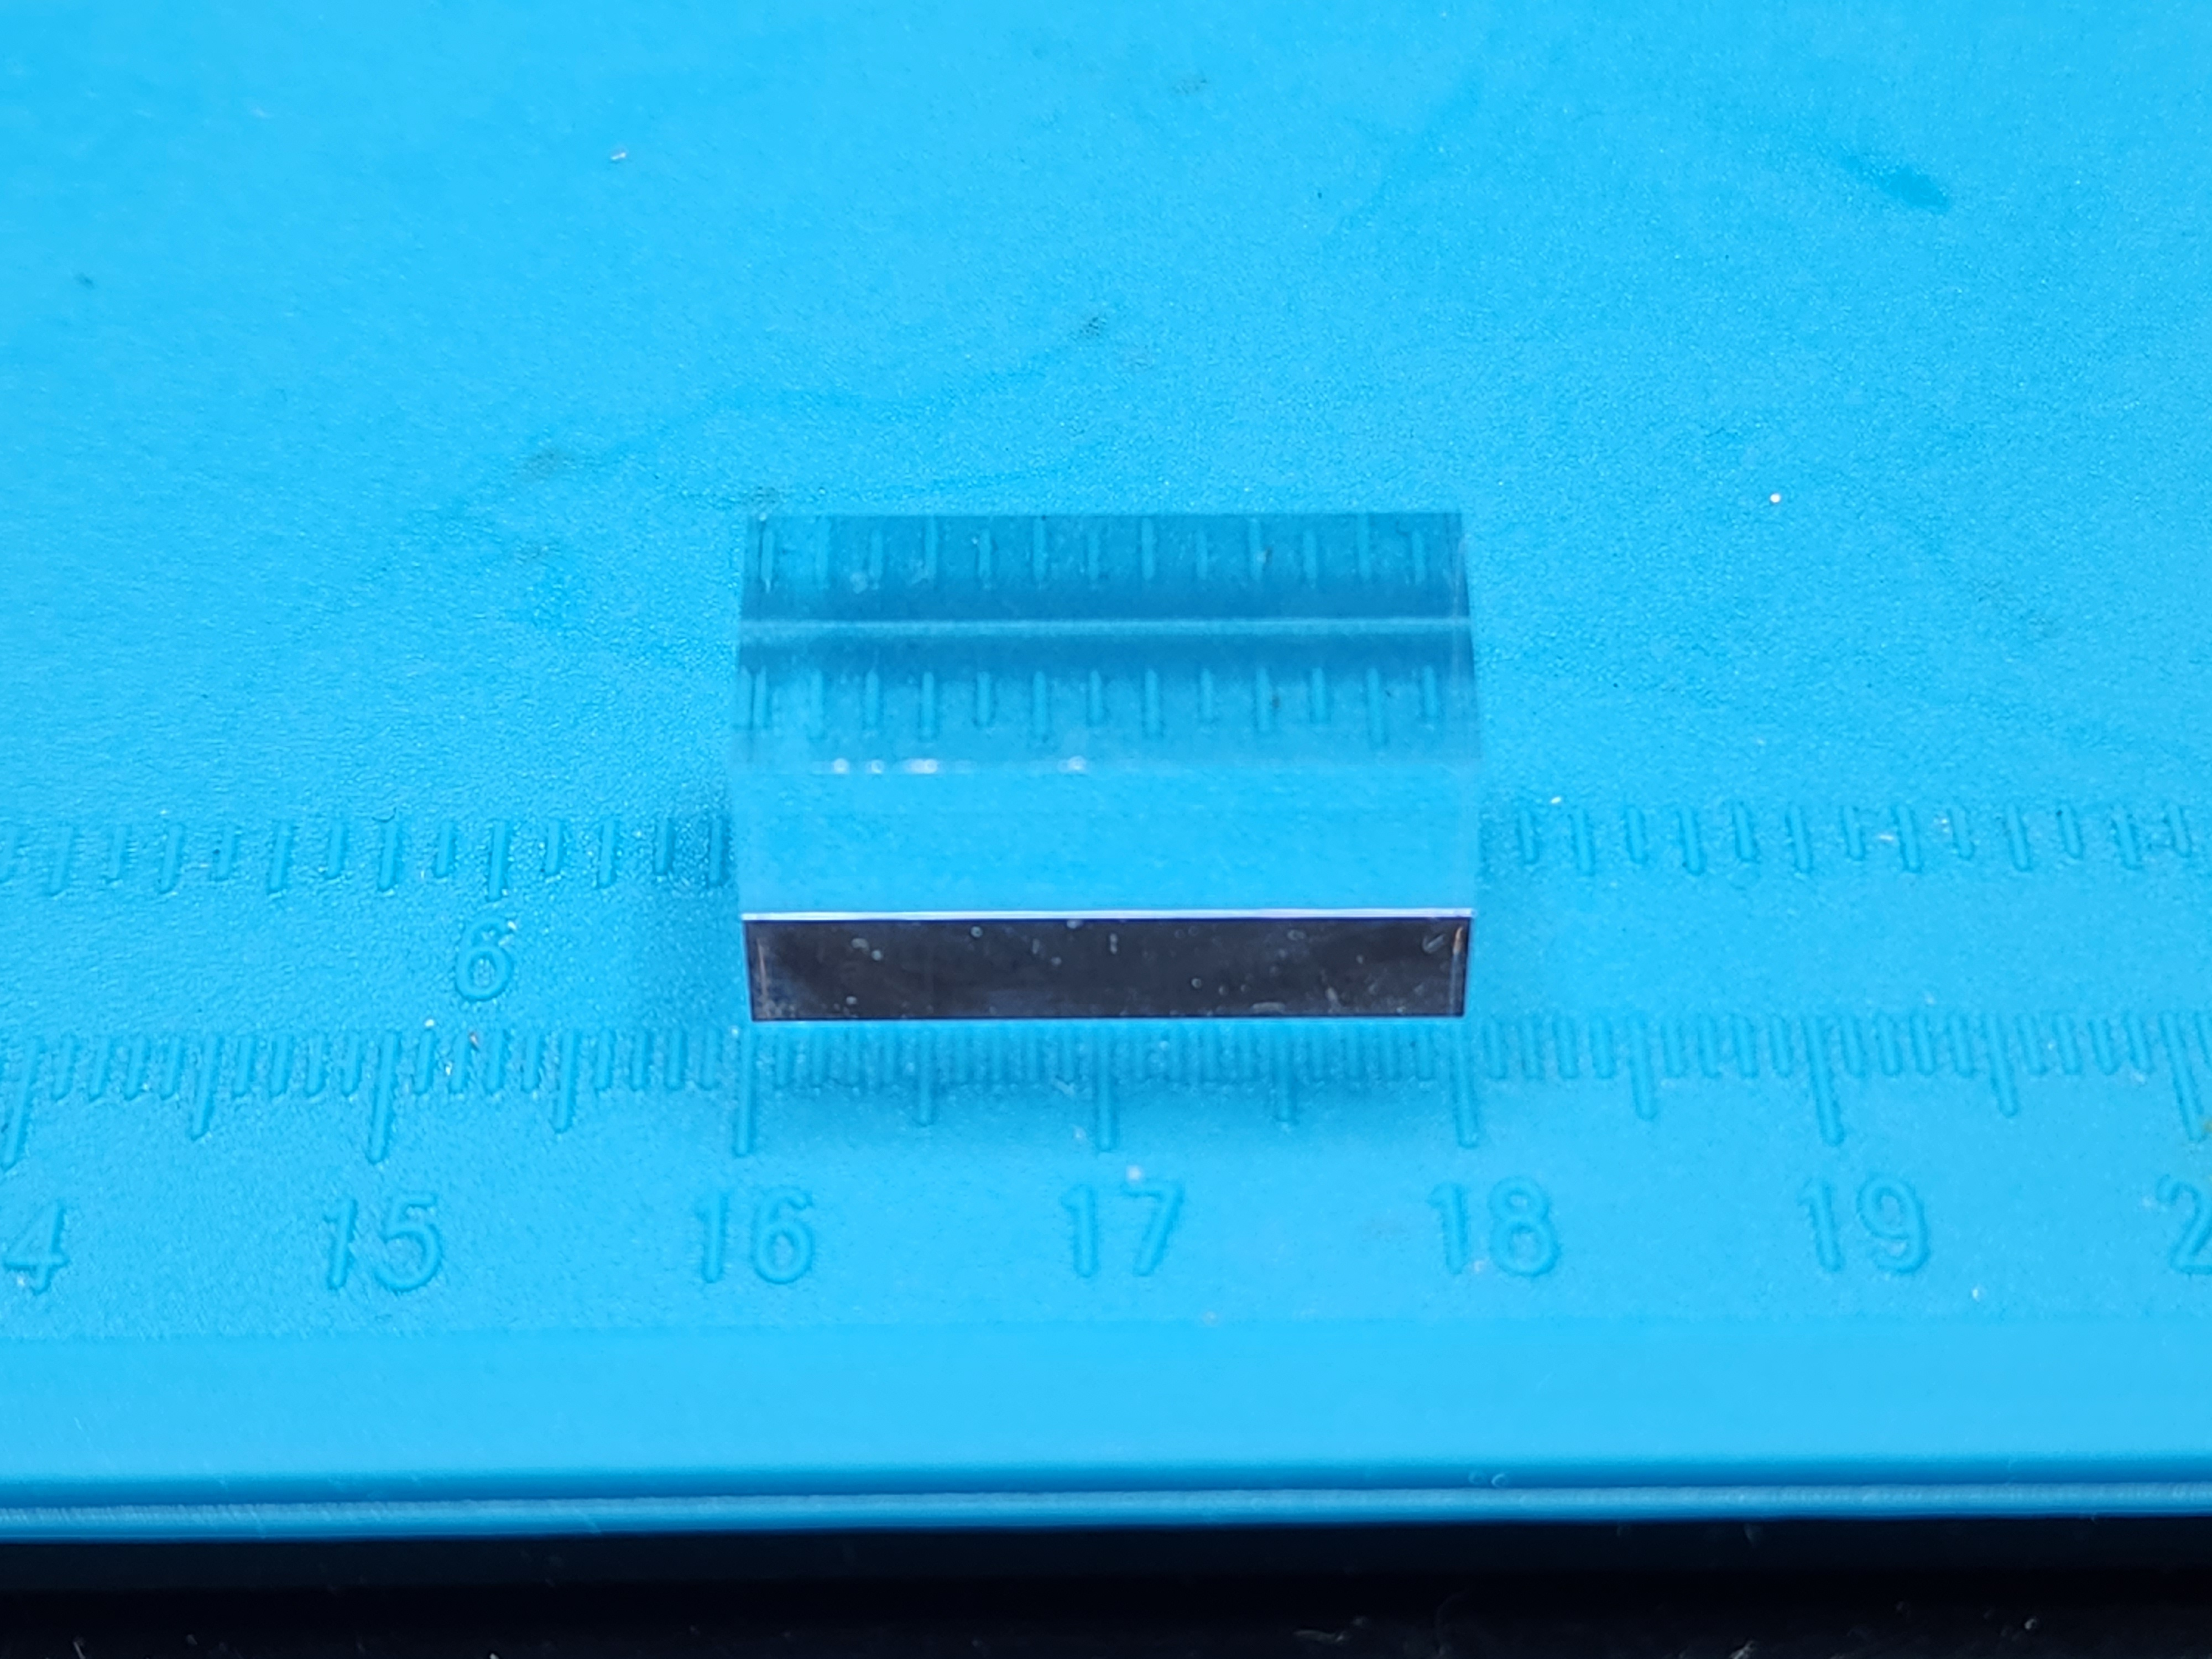
\includegraphics[width=\textwidth]{measurements/LYSO_crystals/LYSO_20_10_10.jpg}
  \end{subfigure}
  \begin{subfigure}[t]{0.49\textwidth}
    \centering
    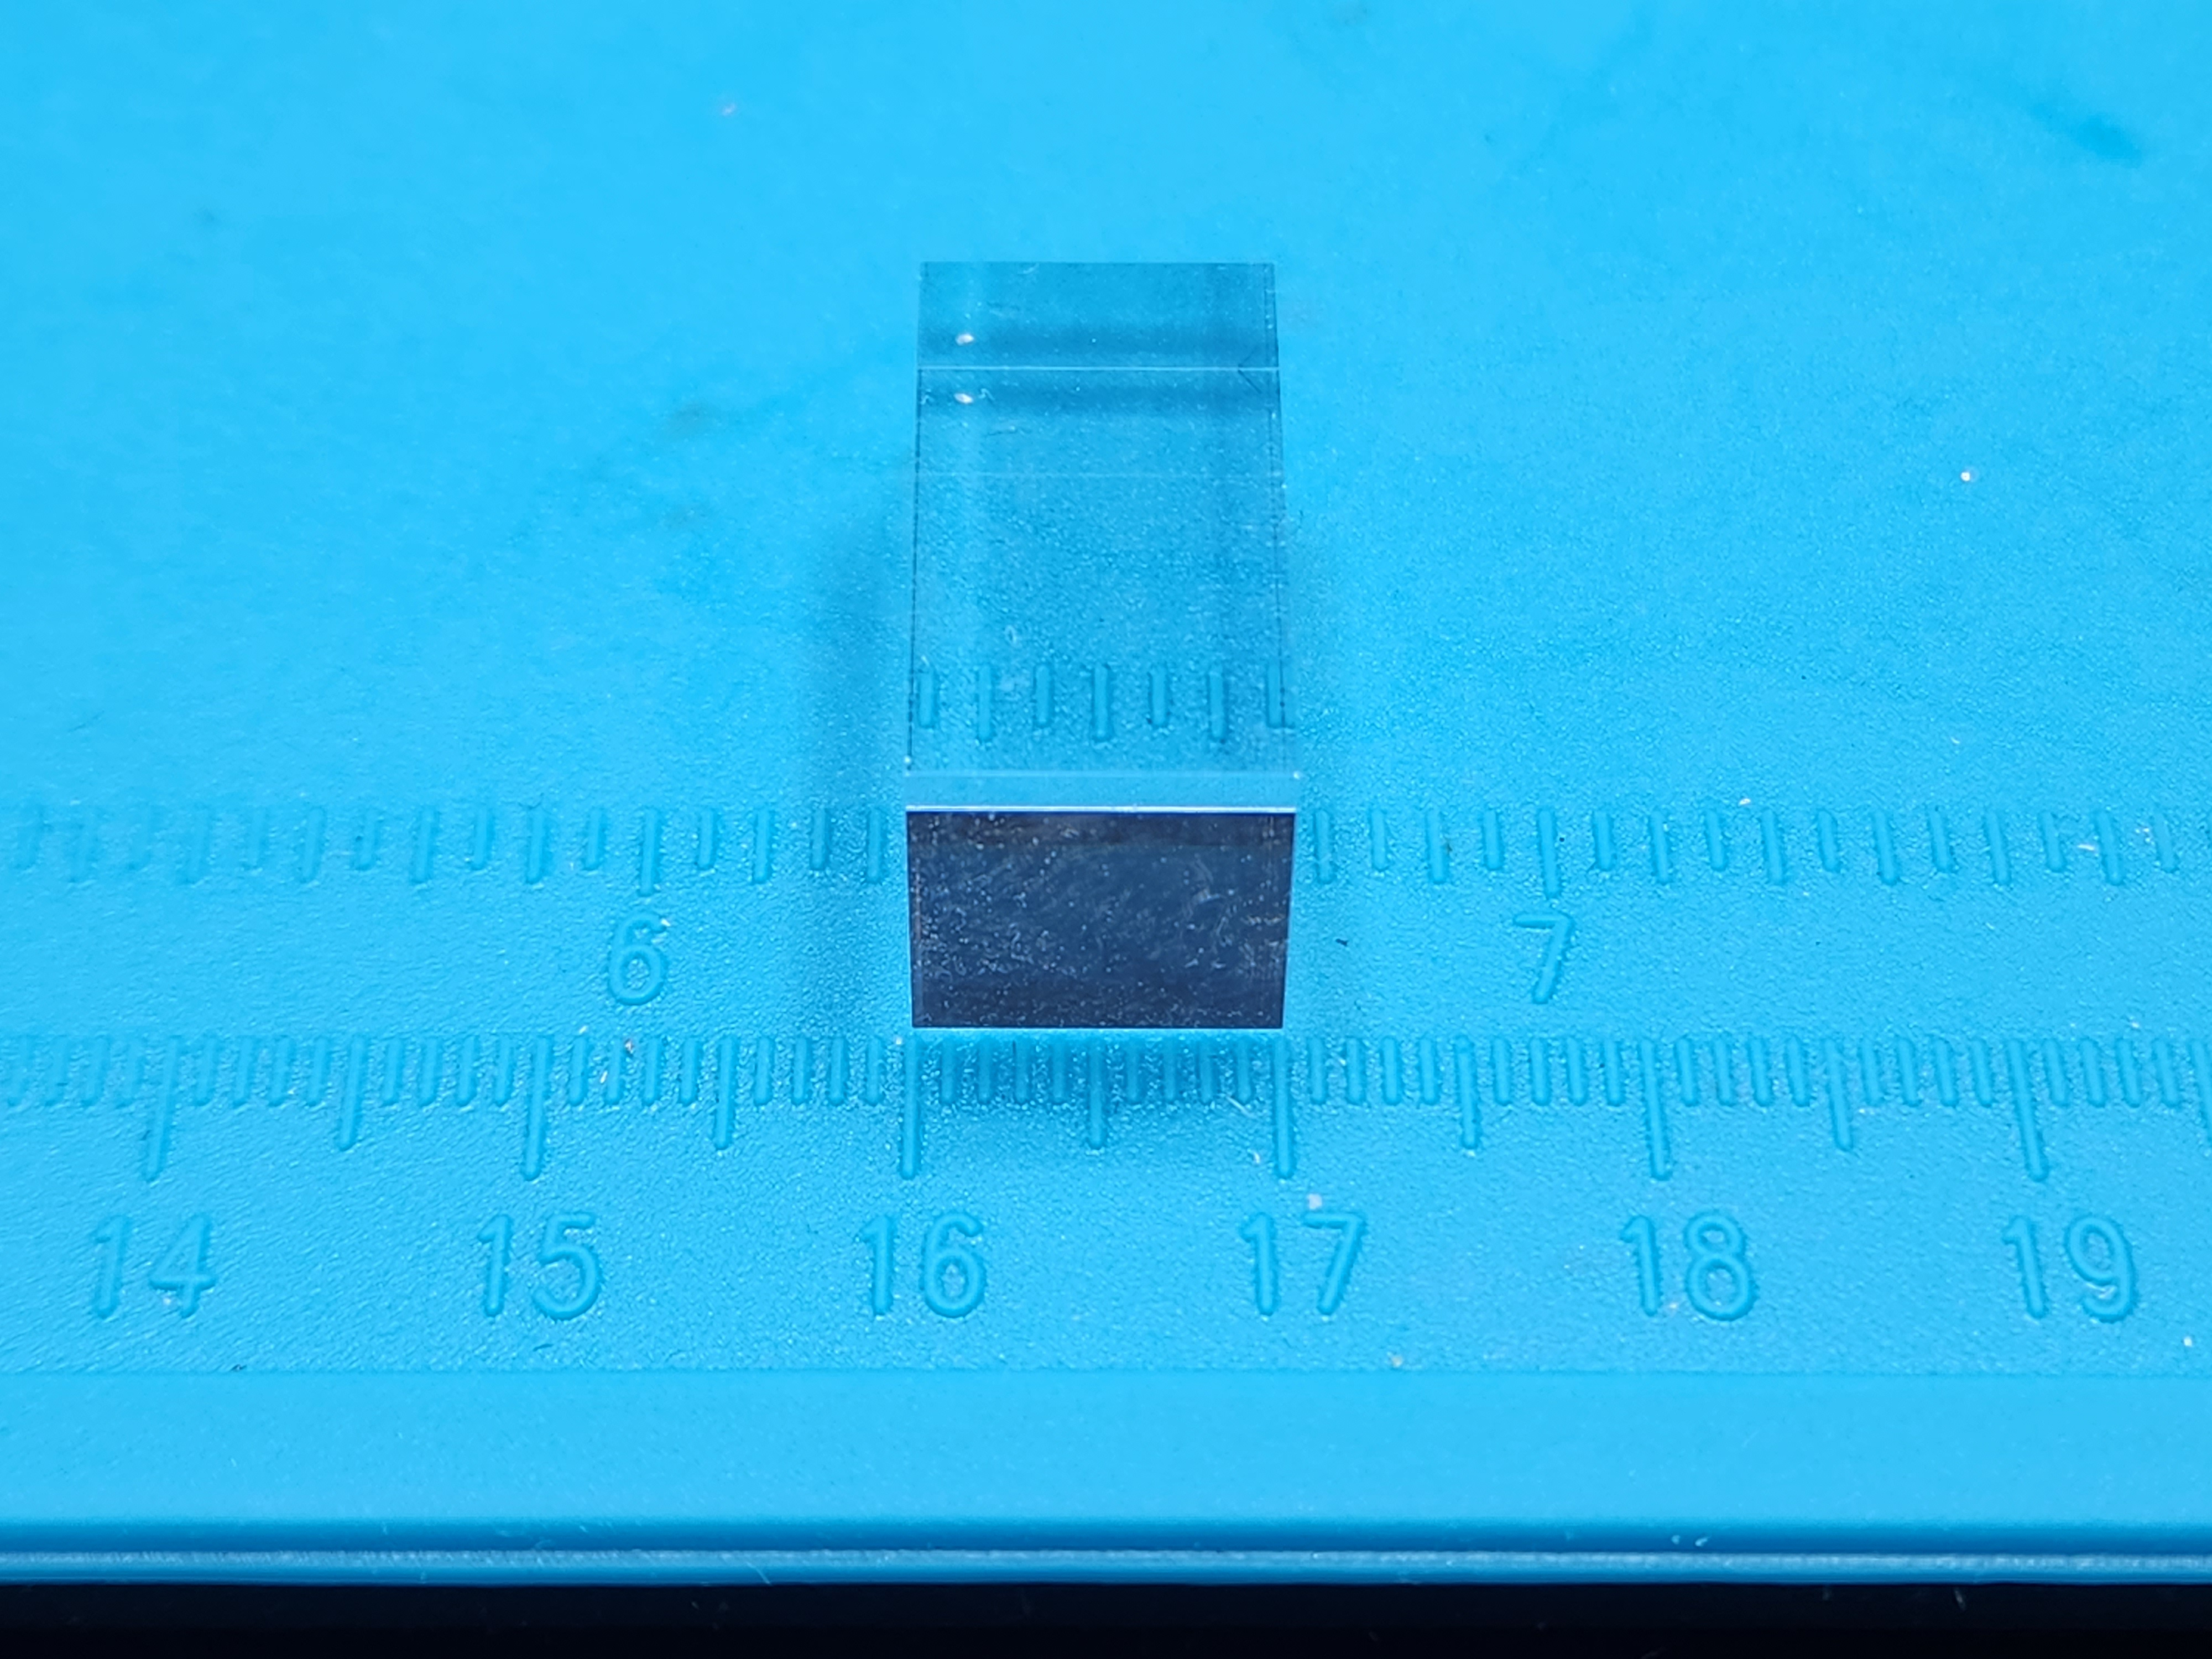
\includegraphics[width=\textwidth]{measurements/LYSO_crystals/LYSO_20_10_10_2.jpg}
  \end{subfigure}
  \medskip
  \begin{subfigure}[t]{\textwidth}
    \centering
    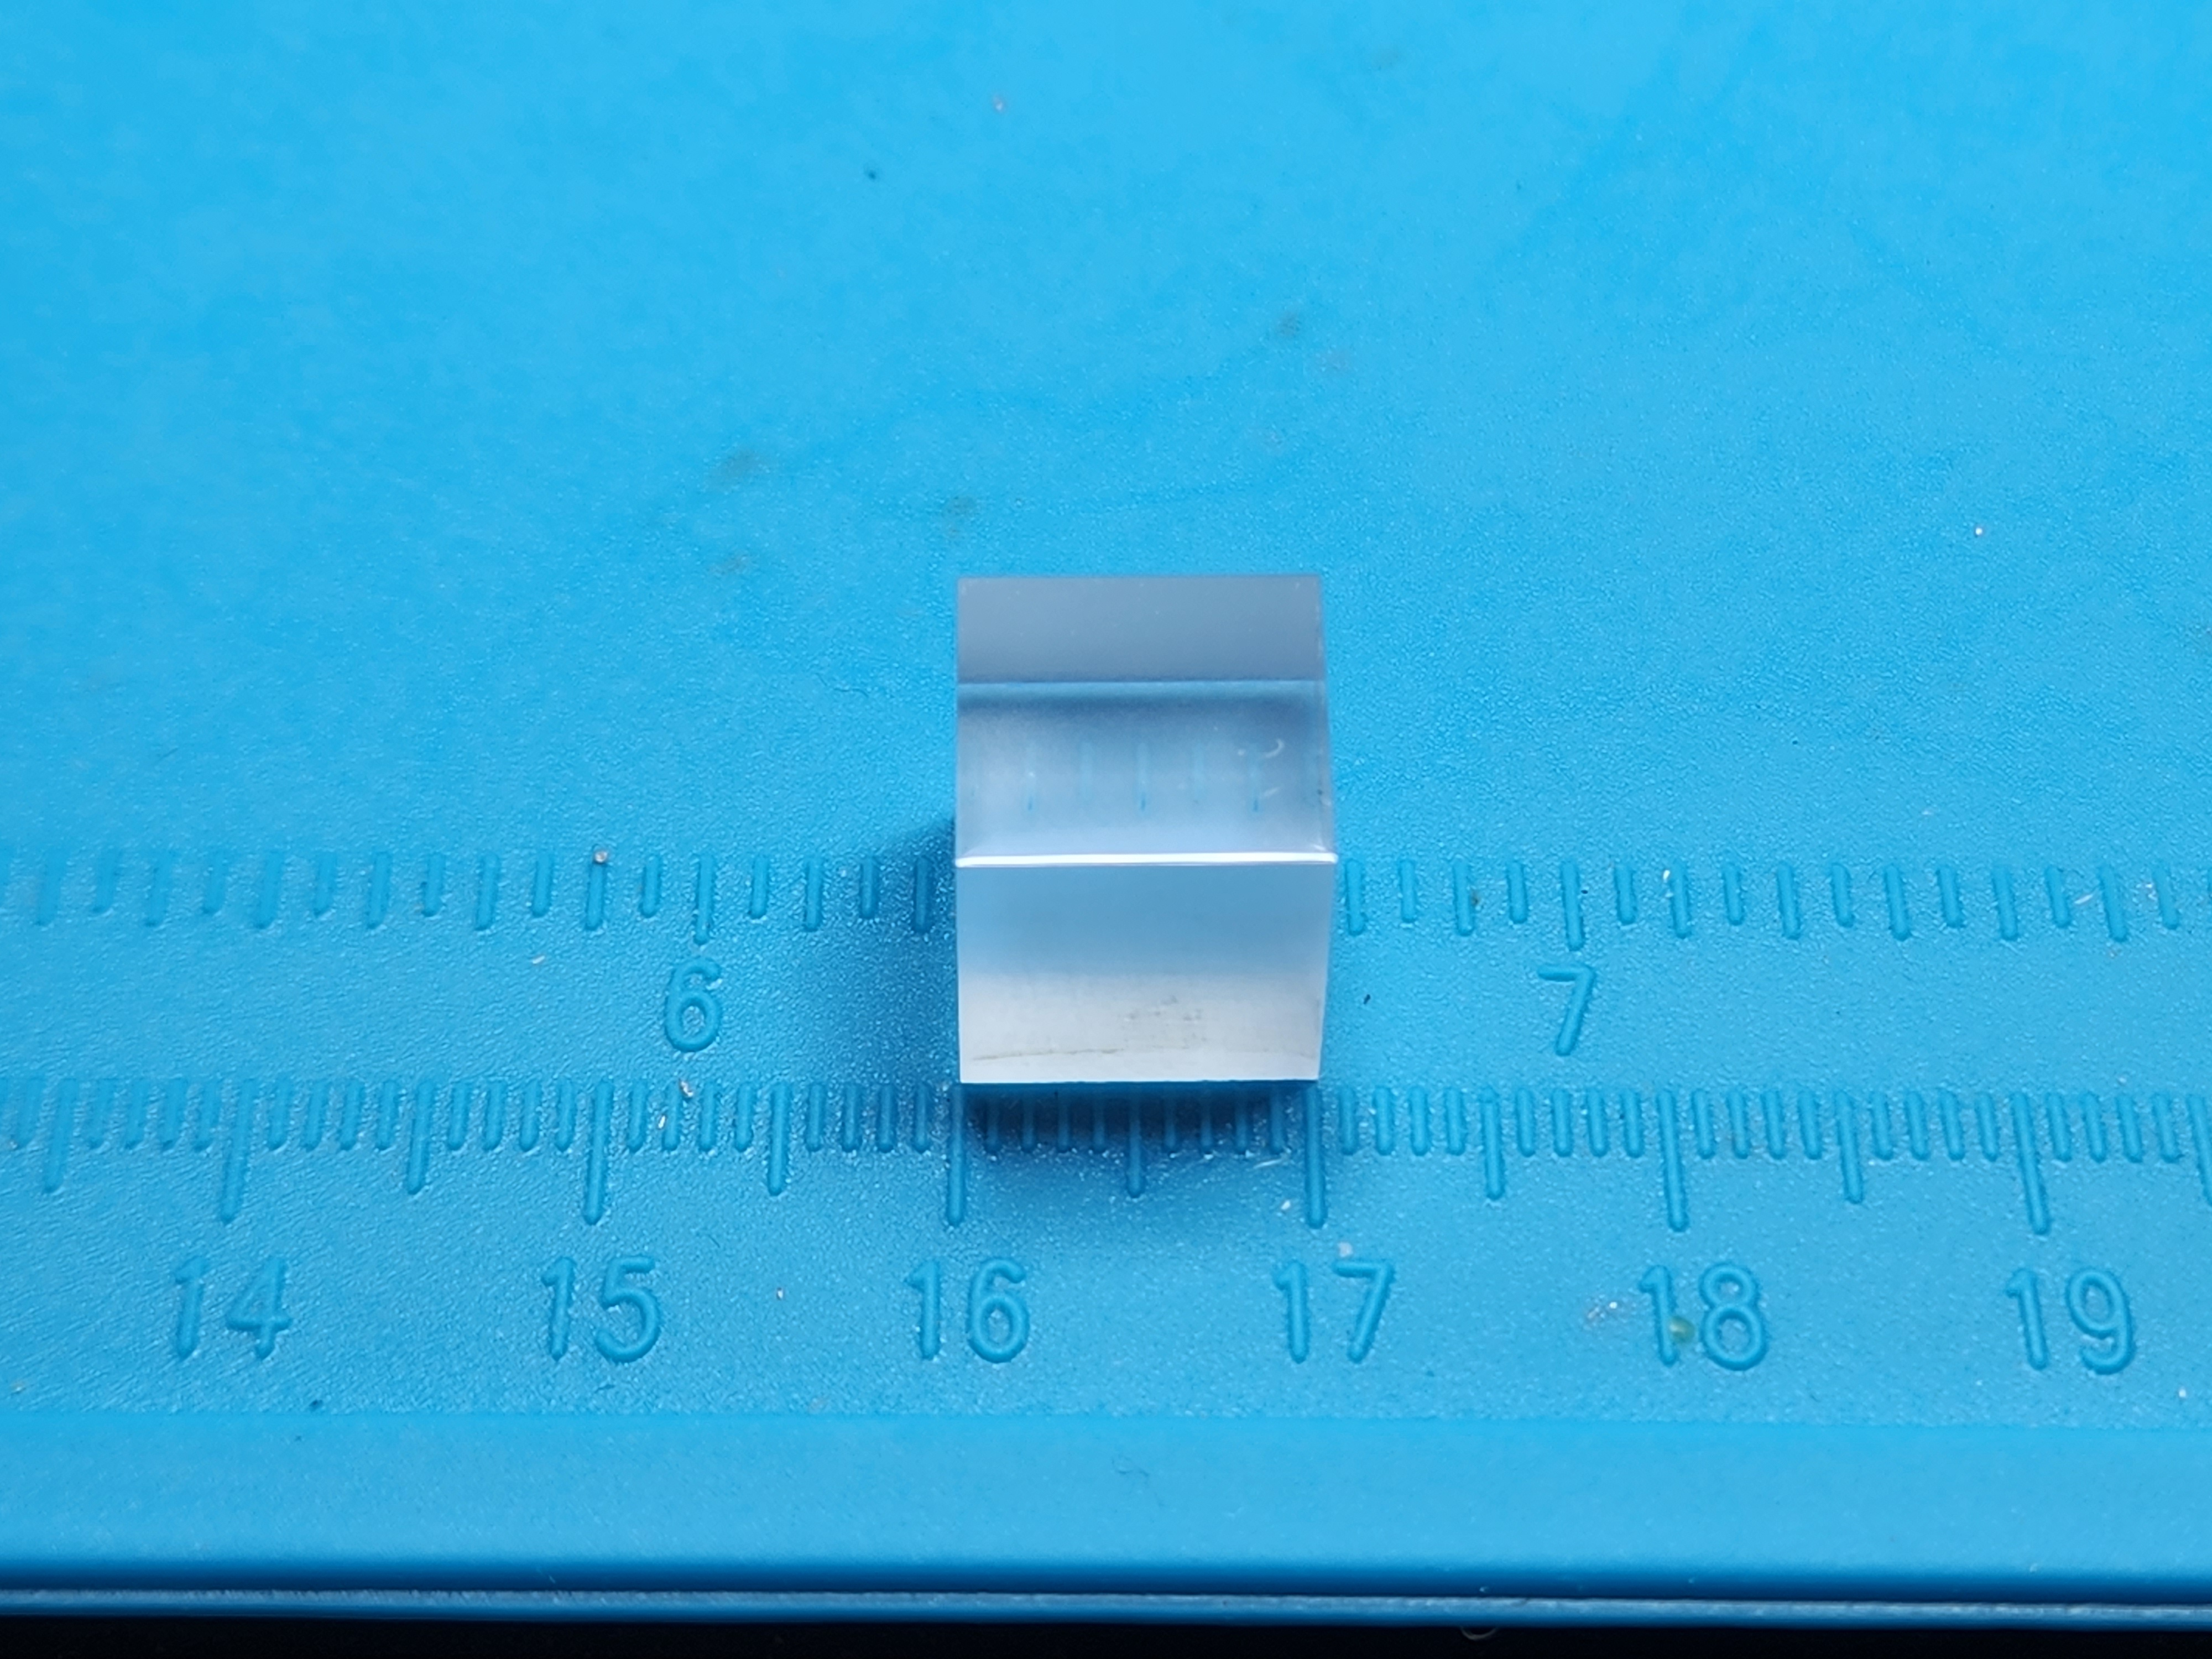
\includegraphics[width=0.5\textwidth]{measurements/LYSO_crystals/LYSO_10_10_10.jpg}
  \end{subfigure}
  \caption{\label{fig:LYSO_crystals}Dimensions of LYSO crystals used to test the CosmicWatch response.}
\end{figure}